\documentclass{article}
\usepackage{blindtext}
\usepackage[letterpaper,top=2cm,bottom=2cm,left=3cm,right=3cm,marginparwidth=1.75cm]{geometry}
\usepackage{graphicx}
\usepackage[colorlinks=true, allcolors=blue]{hyperref}
\usepackage{mathptmx}
\usepackage{tikz}
\usetikzlibrary{calc}


\graphicspath{ {./images/} }

\title{OCOPEE - Online Expo Center}
\author{Tran Ngoc Huy\\[1cm]{\small Advisor: PhD. Le Thi My Hanh}}
 
\date{\today}

\begin{document}
%========================================================= %
%================begin of title page====================== %
% The frontmatter environment for everything that comes with roman numbering\
%============================================= %

	%%%%%%%%%%%%%%%%%%%%%%%%%%%%%%%%%%%%%%%%%%%%%%%%%%%%%%%%%%%%%%%%%%%
	\begin{titlepage}
		%\AddToShipoutPictureBG
		\begin{center}
		{\large 	THE UNIVERSITY OF DANANG
			
			DANANG UNIVERSITY OF SCIENCE AND TECHNOLOGY
			
			FACULTY OF INFORMATION TECHNOLOGY}
\\[1.3cm]
\begin{figure}[h]  %h means here other options t , b, p, etc.

					\centering
					
\includegraphics[width=0.3\linewidth]{./logo}
					\\[0.8cm]
\end{figure}


{\Huge GRADUATION PROJECT THESIS}
\\[0.8cm]
{\large MAJOR: .................................................}

{\large SPECIALTY: .......................................}
\\[1.5cm]
PROJECT TITLE:
\\[0.5cm]

{\huge OCOPEE - ONLINE EXPO CENTER}
\\[1.5cm]
{\large 
	Instructor: PhD. Le Thi My Hanh

	Student: Tran Ngoc Huy

	Student ID: 102180208

	Class: 18TCLC\_DT3
}
\\[5.5cm]
Da Nang, ...../201...
		
		\end{center}
	\end{titlepage}
	
	%----------------------ACKNOWLEDGEMENT---------------------------
	\pagenumbering{gobble}
	\pagebreak
	\newpage
	\pagenumbering{roman}
	\setcounter{page}{1}
	\newpage
	\tableofcontents
	\listoffigures
	%\newpage
	
	%================================================ %
	% The frontmatter environment for everything that comes with roman numbering %

%%%%%%%%%%%%%%%%%%%%%%%%%%%%%%%%%%%%%%%

\newpage
\pagenumbering{arabic}


%%%%%%%%% MAIN TEXT STARTS HERE %%%%%%%%%%
	\section{Introduction}
	"Now there are many directions of development. Most are plans, strategies or are in the process of being tested. But there is one thing I have said over and over again: There are only two sectors that are the future of the Vietnamese economy: the Information Technology sector and the Agriculture sector." - PhD. Alan Phan
	\subsection{Problem}
	Start-up innovation in agriculture and handicrafts approach a new customer hardly. 
	One of the most highly effective channels is Expo Center.
	However, if some environmental reasons prevent an expo from being held, maybe there is no alternative.
	\subsection{Orientation}
	OCOPEE was extended from a classic e-commerce platform to bring a user experience from a usual expo to an online expo. Although it is difficult, it is also an opportunity to help the traditional form of fairs no longer be limited geographically.
	\section{Analysic}
	\subsection{Resources of the system}
	There are some resources that are necessary to create value for the customer.
	\begin{itemize}
		\item Real-time, live-stream system.
		\item Interaction as a social network.
		\item Customer data.
	\end{itemize}
	\subsection{Goals}
	 The most important activities in executing a system's value proposition.
		\begin{itemize}
		\item Community standards, agency policy.
		\item User behavior tracking.
		\item Customer care.
		\item Display shop, product,...
		\item Events, viewer behavior, comments, reactions,...
	\end{itemize}
	\subsection{Features}
	The featues, screens, functions need implement.
	\begin{itemize}
		\item Affiliate marketing for this system can generate a link. The help system can keep track of which customers are invited by the agent.
		\item Register to participate in expo. 
		\item E-commerce function.
		\item Live-stream for business.
		\item Current views counting for shop, product.
		\item Reactions, Comments.
		\item Send quick question in current expo.
	\end{itemize}
	\section{Technology}
	\subsection{Server Architecture}
	Stateful Authentication, Miro-service, Gateway, GraphQL API.
	\subsection{Client Architecture}
	Micro-frontend, one single page, server side render.
	\subsection{DevOps}
	Reverse Proxy, Load balance, Cache, Process Manager, CI/CD.
	
	\begin{figure}[h]
		\caption{State diagram}
		\centering
		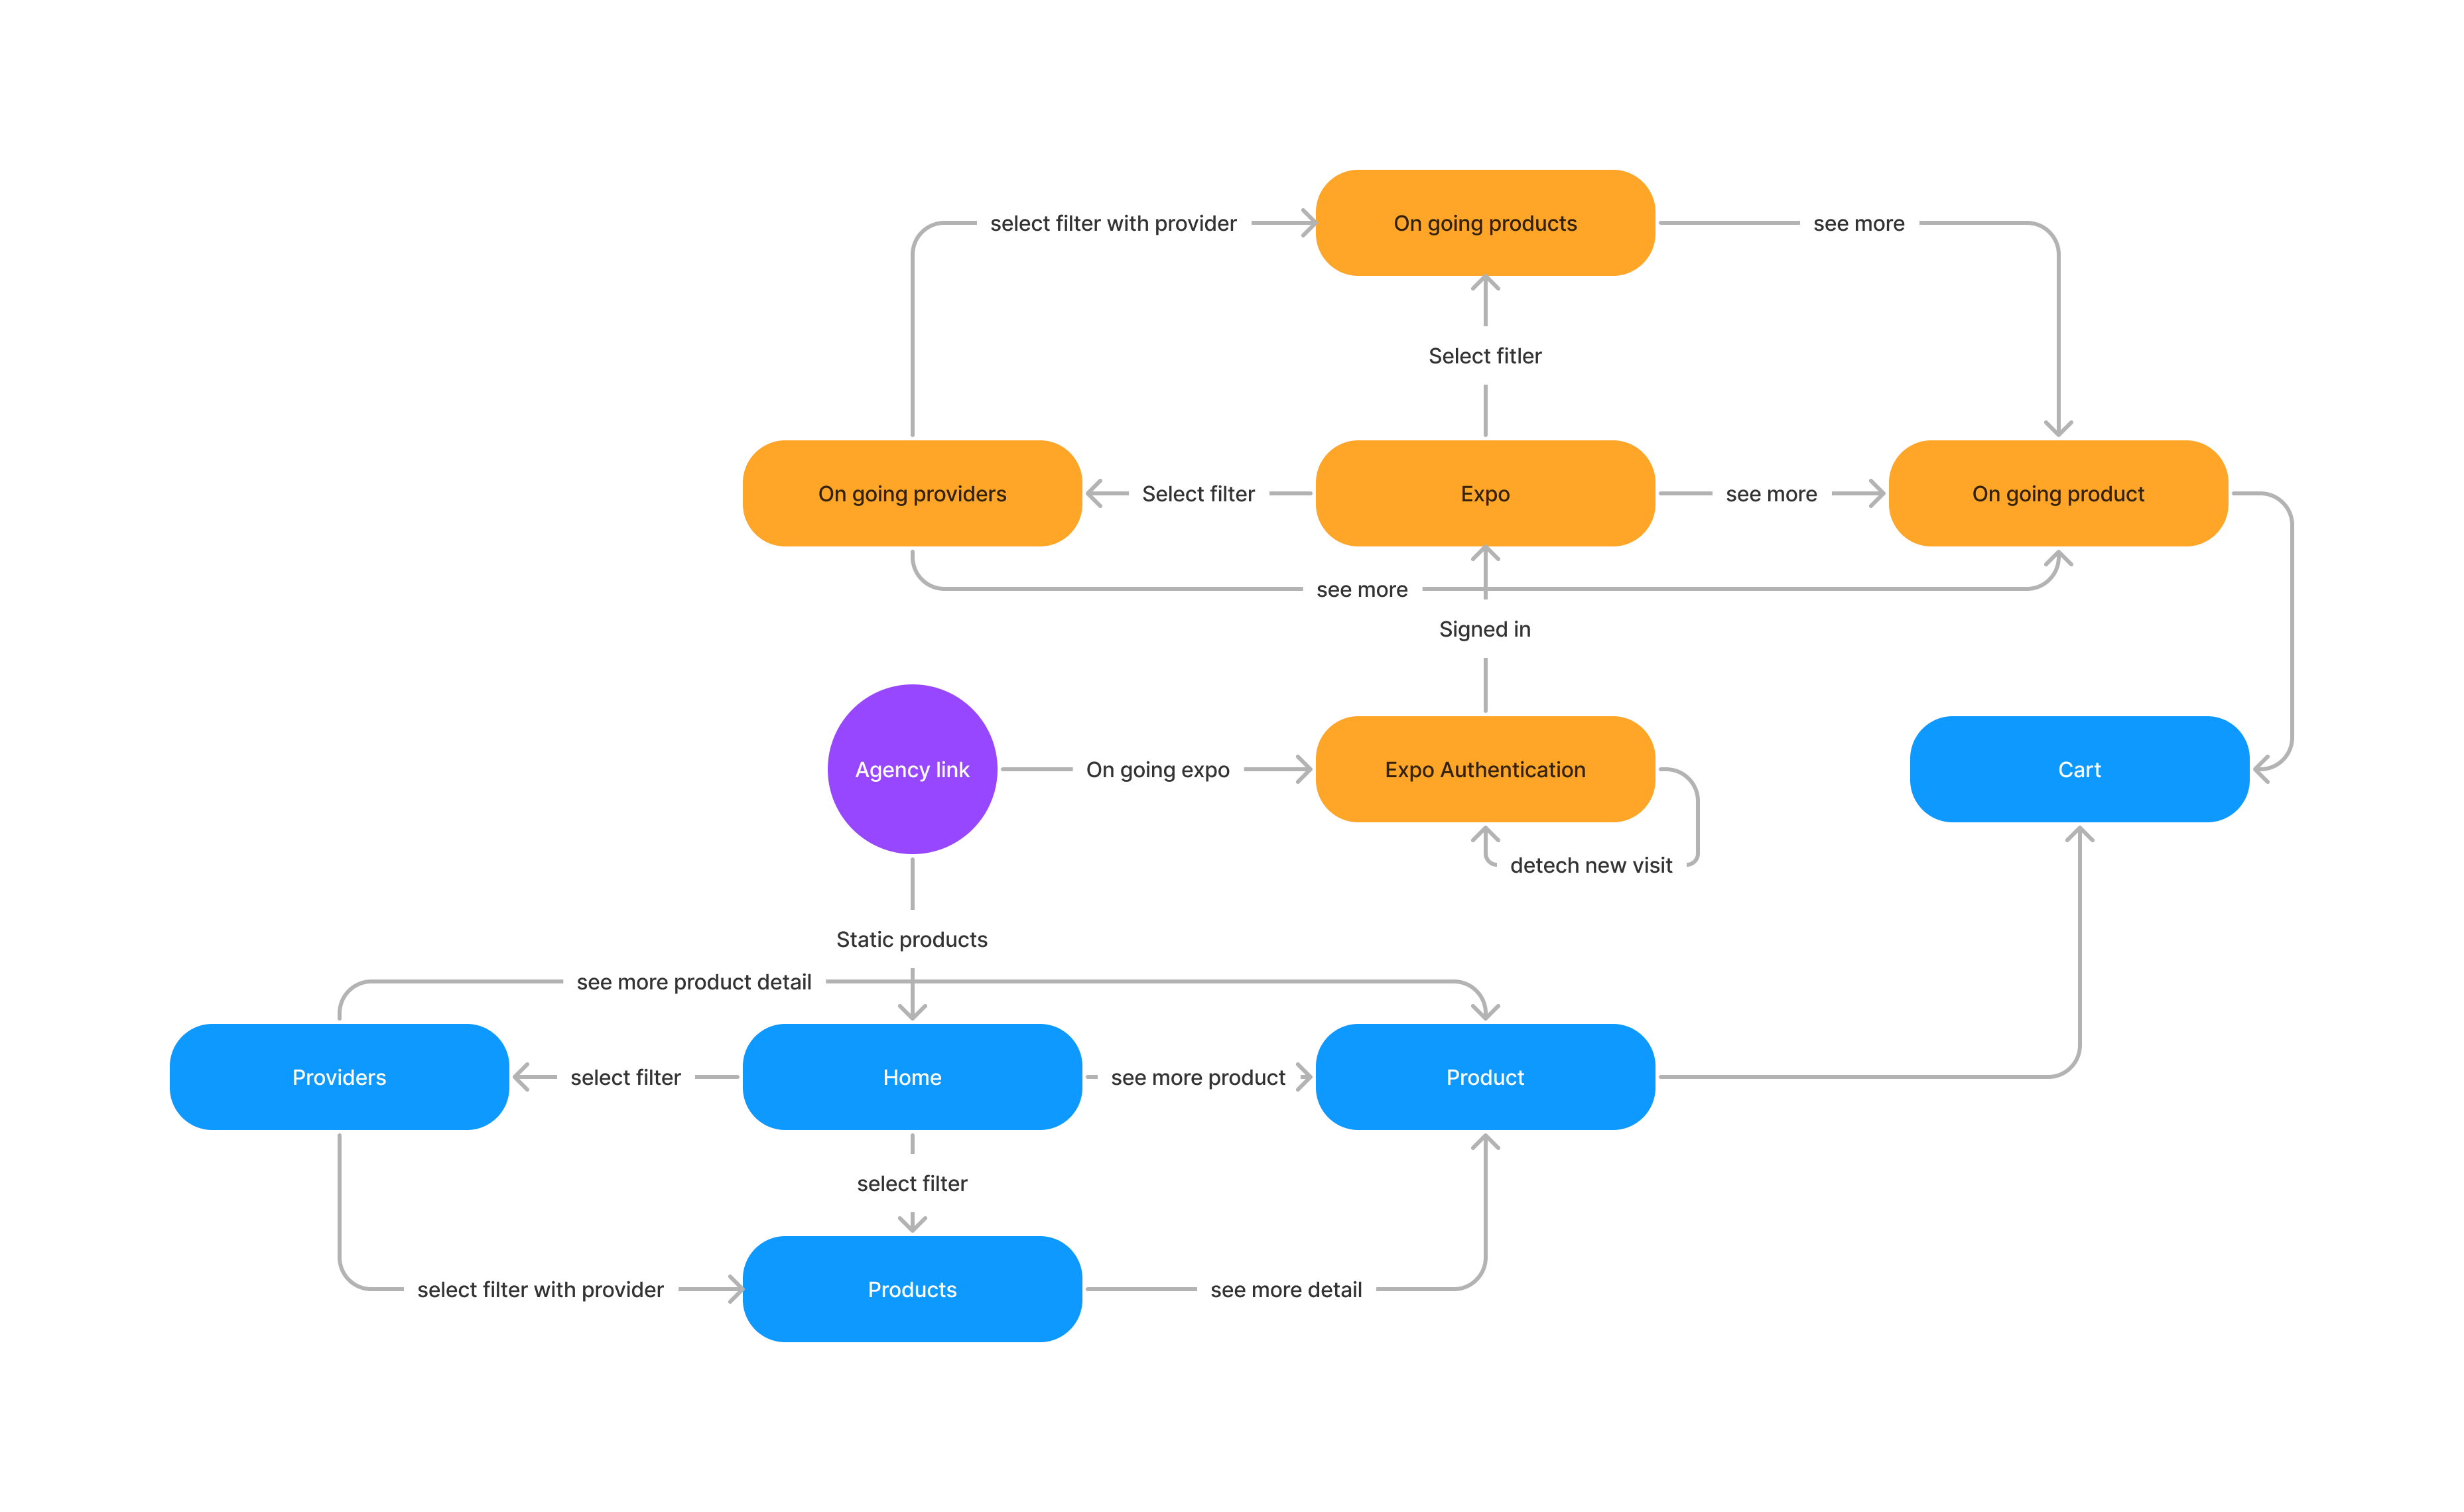
\includegraphics[width=\textwidth]{state.png}
		\label{fig:state}
	\end{figure}
	As you can see in the figure \ref{fig:state}, the function grows near 0. Also, in the page \pageref{fig:state} is the same example.\pageref{fig:state}
	


	
\bibliographystyle{alpha}
\bibliography{sample}

\end{document}